\documentclass{article}

\usepackage[margin=1in]{geometry}
\usepackage{amsmath}
\usepackage{amsfonts}
\usepackage{graphicx}
\usepackage{float}
\usepackage{caption}

\title{Homework 2: Digital Control (ECEN 5458)}
\author{Zachary Vogel}
\date{\today}

\newcommand{\rank}{\text{rank}}

\begin{document}
\maketitle

\section*{Problem 1}
\subsection*{(a)}
Here we want to calculate the unit-pulse response of the system from problem 4.2.
\[u(k)=u(k-1)+\cfrac{T}{12}(5e(k)+8e(k-1)-e(k-2))\]
Doing this numerically we get:
\[u(0)=0+\cfrac{T}{12}(5+0-0)=\cfrac{5T}{12}\]
\[u(1)=\cfrac{5T}{12}+\cfrac{T}{12}(0+8-0)=\cfrac{13T}{12}\]
\[u(2)=\cfrac{13T}{12}+\cfrac{T}{12}(0+0-1)=T\]
\[u(3)=T+0\]
so $u((3,\infty])=T$.
\subsection*{(b)}
Now we want to know if that system is BIBO stable. It is BIBO stable if:
\[\sum_{k=-\infty}^\infty\lvert u(k)\rvert <\infty\]
which is only true if $T=0$, so no it isn't.

\section*{Problem 2}
Given the transfer function:
\[\frac{U(z)}{E(z)}=D(z)=\cfrac{2z}{(z+\frac{1}{2})(z+\frac{1}{3})}\]
\subsection*{(a)}
Draw a block diagram corresponding to this system in control canonical form. Define the state vector $\boldsymbol{x}$, and give the corresponding state matrices $\boldsymbol{A_c}$, $\boldsymbol{B_c}$, $\boldsymbol{C_c}$, and $\boldsymbol{D_c}$.\\
Here is the block diagram:
\begin{figure}[H]
    \centering
    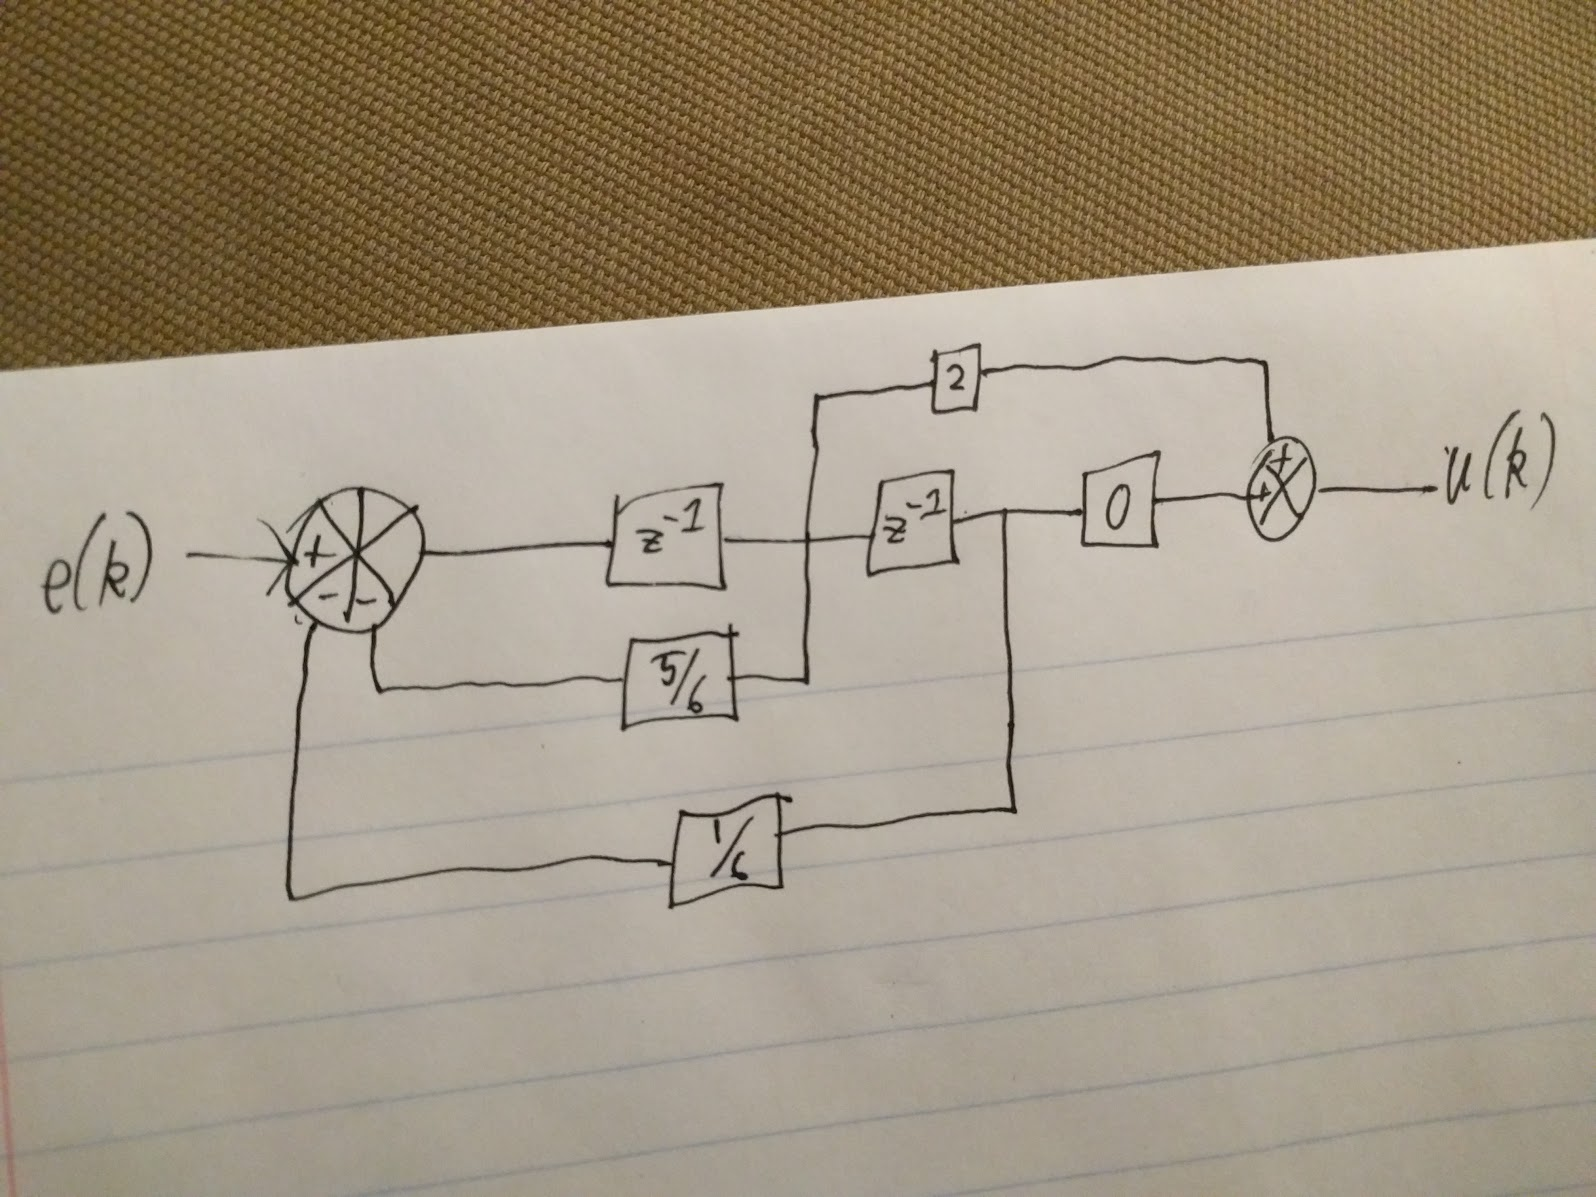
\includegraphics[width=0.9\textwidth]{PR1.jpg}
\end{figure}
Let's define some states:
\[U=2zX,\quad z^2X=E-\frac{5}{6}z-\frac{1}{6}\]
converting back to the discrete domain we get:
\[u(k)=2x(k+1),\quad x(k+2)=-\frac{5}{6}x(k+1)-\frac{1}{6}x(k)+e(k)\]
now define $x(k)=x_2(k)$ and $x_1(k)=x_2(k+1)$ this gives:
\[\begin{bmatrix}x_1(k+1)\\x_2(k+1)\end{bmatrix}=\begin{bmatrix}-\frac{5}{6} &-\frac{1}{6}\\1&0\end{bmatrix}\begin{bmatrix}x_1(k)\\x_2(k)\end{bmatrix}+\begin{bmatrix}1\\0\end{bmatrix}e(k)\]
\[u(k)=\begin{bmatrix}2&0\end{bmatrix}\begin{bmatrix}x_1(k)\\x_2(k)\end{bmatrix}+0*e(k)\]
Thus we have our controllable canonical form matrices.
\subsection*{(b)}
Write the transfer function $D(z)$ in the following form:
\[D(z)=\cfrac{c_a}{z+\frac{1}{2}}+\cfrac{c_b}{z+\frac{1}{3}}\]
Then, draw a block diagram representing this system in controllable canonical form. Then define the state $\bar{\boldsymbol{x}}$ and give the state matrices $\bar{\boldsymbol{A}}$, $\bar{\boldsymbol{B}}$, $\bar{\boldsymbol{C}}$, and $\bar{\boldsymbol{D}}$.\\
Immediately:
\[2z=c_a(z+\frac{1}{3})+c_b(z+\frac{1}{2})\]
\[c_a+c_b=2,\quad \frac{c_a}{3}+\frac{c_b}{2}=0\]
solving these yields $c_a=6$ and $c_b=-4$. Here is the block diagram.
\begin{figure}[H]
    \centering
    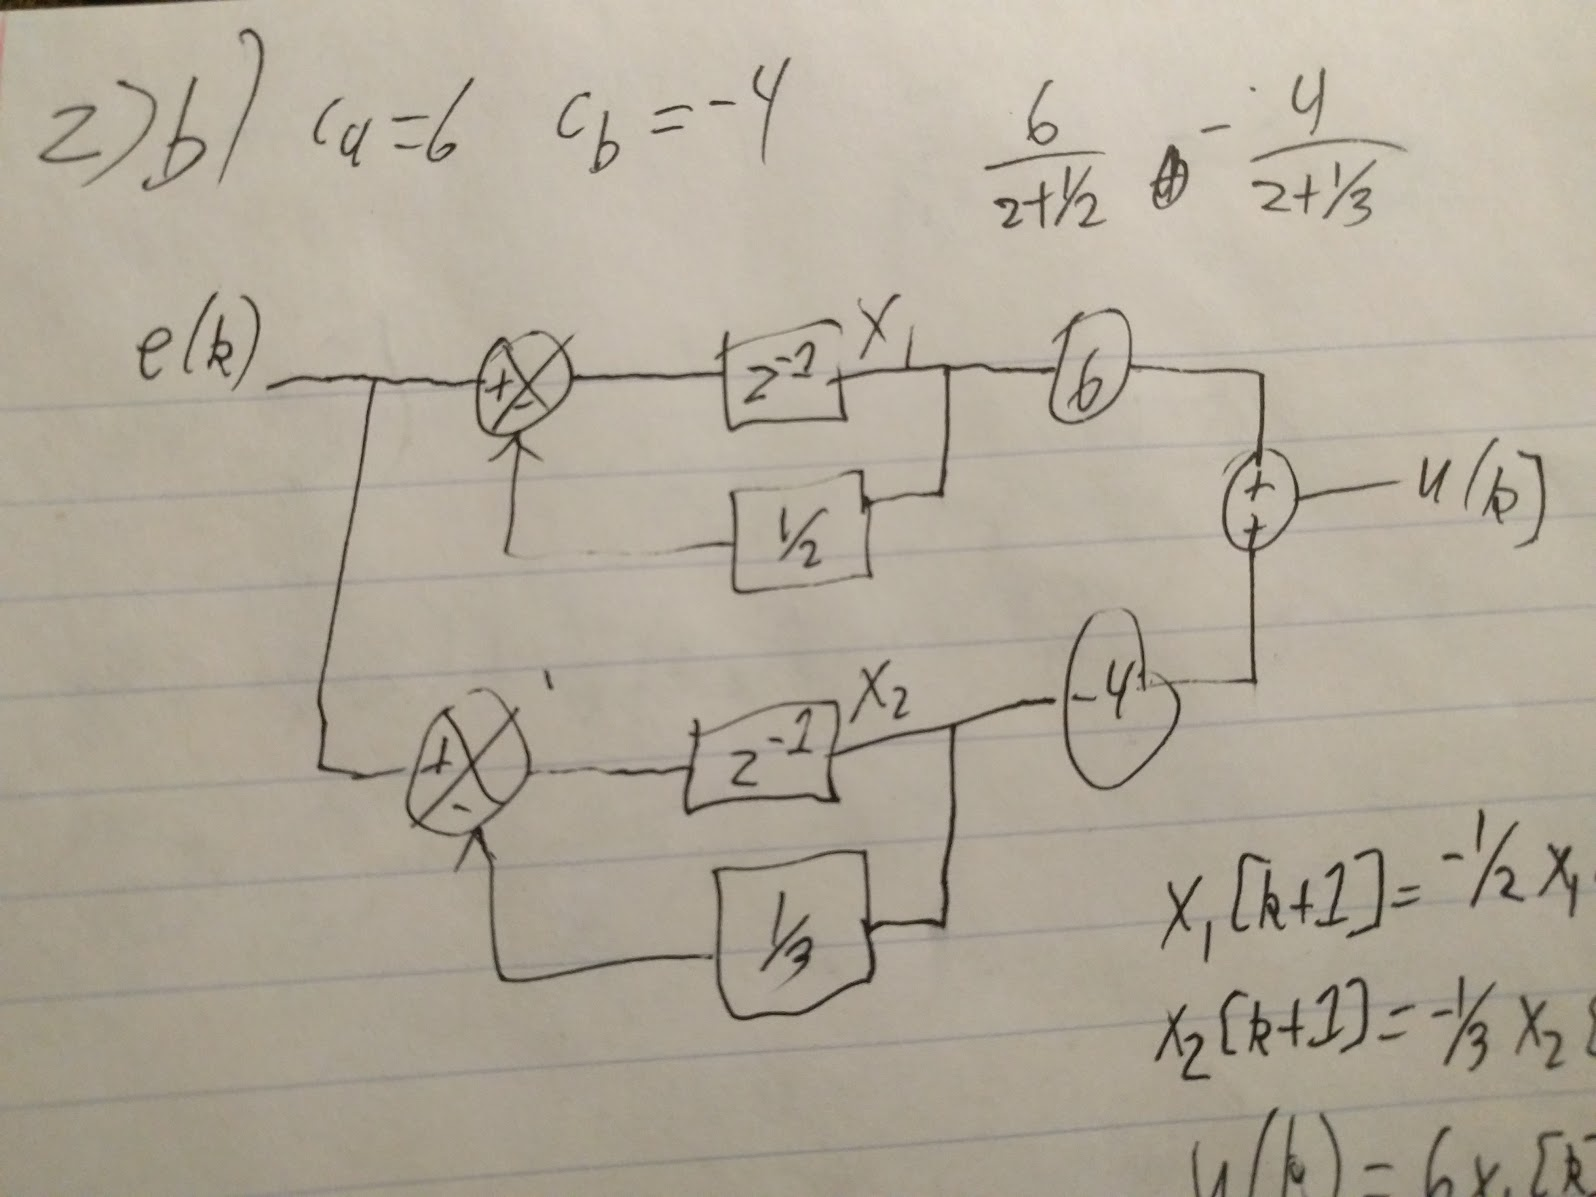
\includegraphics[width=0.9\textwidth]{PR2.jpg}
\end{figure}
Then, we define our states $\bar{\boldsymbol{x}}$:
\[X_1(z)=\frac{1}{z+\frac{1}{2}}E(z)\]
\[X_2(z)=\frac{1}{z+\frac{1}{3}}E(z)\]
\[U(z)=6X_1-4X_2\]
Then converting back to the digital time domain we get:
\[\bar{x_1}(k+1)=-\frac{1}{2}\bar{x_1}(k)+e(k)\]
\[\bar{x_2}(k+1)=-\frac{1}{3}\bar{x_2}(k)+e(k)\]
\[u(k)=6\bar{x_1}(k)-4\bar{x_2}(k)\]
Our matrices are:
\[\bar{\boldsymbol{A}}=\begin{bmatrix}-\frac{1}{2}&0\\0&-\frac{1}{3}\end{bmatrix}\]
\[\bar{\boldsymbol{B}}=\begin{bmatrix}1\\1\end{bmatrix}\]
\[\bar{\boldsymbol{C}}=\begin{bmatrix}6&-4\end{bmatrix}\]
and $\bar{\boldsymbol{D}}=0$.

\subsection*{(c)}
Find the transfer functions $\frac{X_1(z)}{E(z)}$ and $\frac{X_2(z)}{E(z)}$ from the state matrices in part (a). Expand these into partial fraction form and express $x_1$ and $x_2$ in terms of $\bar{x}_1$ and $\bar{x}_2$. Then find the transformation matrix such that $\boldsymbol{x}=\boldsymbol{T}\bar{\boldsymbol{x}}$.\\
Here we have the states from part a:
\[\cfrac{X_1}{E}=\cfrac{zX_2}{E}=\cfrac{z}{z^2+\frac{5}{6}z+\frac{1}{6}}\]
we get two equations for both $x_1$ and $x_2$:
\[x_1,\quad A+B=1,\quad \frac{A}{3}+\frac{B}{2}=0\]
\[x_2,\quad C+D=0,\quad \frac{C}{3}+\frac{D}{2}=1\]
This gives $A=3,B=-2,C=-6,D=6$. Our transition matrix is:
\[T=\begin{bmatrix}3 &-2\\-6&6\end{bmatrix}\]

\subsection*{(d)}
Verify that the transformation matrix found in part (c) holds for the following formulas:
\[\bar{\boldsymbol{A}}=\boldsymbol{T}^{-1}\boldsymbol{A}_c\boldsymbol{T},\quad \bar{\boldsymbol{B}}=\boldsymbol{T}^{-1}\boldsymbol{B}_c,\quad \bar{\boldsymbol{C}}=\boldsymbol{C}_c\boldsymbol{T},\quad \bar{\boldsymbol{D}}=\boldsymbol{D}_c\]
First, $T^{-1}$ is:
\[T^{-1}=\begin{bmatrix}1&\frac{1}{3}\\1&\frac{1}{2}\end{bmatrix}\]
D is obviously correct.
\[T^{-1}A_cT=\begin{bmatrix}-0.5&0\\0&-\frac{1}{3}\end{bmatrix}\]
\[T^{-1}B_c=\begin{bmatrix}1\\1\end{bmatrix}\]
\[C_cT=\begin{bmatrix}6&-4\end{bmatrix}\]
All correct, checked with octave.


\section*{Problem 3}
Given the following discrete time plant:
\[G(z)=\cfrac{Y(z)}{U(z)}=\cfrac{z+\frac{1}{2}}{(z-\frac{1}{3})(z-\frac{1}{4})}=\cfrac{z+\frac{1}{2}}{z^2-\frac{7}{12}z+\frac{1}{12}}\]
\subsection*{(a)}
Write a difference equation relating the input $u(k)$ to the output $y(k)$. Without using state space representation, this is fairly easy to do.
\[Y(z)(z^2-\frac{7}{12}z+\frac{1}{12})=U(z)(z+\frac{1}{2})\]
\[y[k]-\frac{7}{12}y[k-1]+\frac{1}{12}y[k-2]=u[k-1]+\frac{1}{2}u[k-2]\]
\subsection*{(b)}
Of the four shown block diagrams on the next page, which one is a correct representation of $G(z)$? Provide any computations and reasoning for your answer.\\
After some analysis, I can confirm that the only correct block is figure 3. Figure 1 is close, needing a sign flip on the feedback. Figure 2 and 4 are wholly inaccurate. Here is the math I did to show that block diagram 3 is correct:
\[\cfrac{Y(z)}{U(z)}=\cfrac{z+\frac{1}{2}}{(z-\frac{1}{3})(z-\frac{1}{4})}=\cfrac{A}{z-\frac{1}{3}}+\cfrac{B}{z-\frac{1}{4}}\]
This leads to the two equations:
\[A+B=1,\quad -\frac{1}{4}A-\frac{1}{3}B=\frac{1}{2}\]
which yields $A=10$ and $B=-9$. Then we define our states with:
\[Y(z)=10X_1(z)-9X_2(z)\]
\[X_1(z)=\cfrac{U(z)}{z-\frac{1}{3}},\quad X_2(z)=\cfrac{U(z)}{z-\frac{1}{4}}\]
This leads to the state equations:
\[x_1[k+1]=\frac{1}{3}x_1[k]+u[k],\quad x_2[k+1]=\frac{1}{4}x_2[k]+u[k]\]
\[y[k]=10x_1[k]-9x_2[k]\]
These equations clearly represent the system in block diagram 3.
\subsection*{(c)}
Defining the states as indicated in the particular block diagram you chose in part (b), write the discrete-time state-space equations for the plant. Thus, we want $\boldsymbol{\Phi}$, $\boldsymbol{\Gamma}$, $\boldsymbol{H}$, and $J$ such that:
\[\begin{array}{c}\boldsymbol{x}(k+1)=\boldsymbol{\Phi}\boldsymbol{x}(k)+\boldsymbol{\Gamma}u(k)\\y(k)=\boldsymbol{H}\boldsymbol{x}(k)+Ju(k)\end{array}\]
where:
\[\boldsymbol{x}(k)=\begin{bmatrix}x_1(k)\\x_2(k)\end{bmatrix}\]
All of this is pretty easy because we already defined our state equations.
\[\boldsymbol{\Phi}=\begin{bmatrix}\frac{1}{3}&0\\0&\frac{1}{4}\end{bmatrix}\]
\[\boldsymbol{\Gamma}=\begin{bmatrix}1\\1\end{bmatrix}\]
\[\boldsymbol{H}=\begin{bmatrix}10&-9\end{bmatrix}\]
and $J=0$.

\section*{Problem 4}
Problem 4.9 (c), (e) and part (h) for parts (c) and (e)\\
This problem asks us to compute $G(z)$ given the following $G(s)$
\subsection*{(c)}
\[G(s)=\cfrac{3}{(s+1)(s+3)}\]
using partial fraction decomposition we get:
\[G(s)=\cfrac{3}{2(s+1)}-\cfrac{3}{2(s+3)}\]
This is then converted to the Z domain:
\[G(z)=\cfrac{3z}{2(z-e^{-T})}-\cfrac{3z}{2(z-e^{-3T})}\]
\subsection*{(e)}
This one is a little trickier.
\[G(s)=\cfrac{e^{\frac{sT}{2}}}{s^2}\]
converting to the time domain we get:
\[g(t)=(t+\frac{T}{2})u(t+\frac{T}{2})\]
we sample at time $kT$ though so there is no functional difference between $u(t+\frac{T}{2})$ and $u(t)$. Thus:
\[g(kT)=(kT+\frac{T}{2})u(kT)\]
which converts to the Z-domain as:
\[G(z)=\cfrac{Tz}{(z-1)^2}+\cfrac{Tz}{2(z-1)}\]

\subsection*{(h)(c)}
Here we use the zpk command to generate the transfer function, Gs=zpk([],[-1 -3],3). Then we use the c2d command with a period of T=0.5, and T=0.05, c2d(Gs,T). The result is:
\[G(z,0.05)=\cfrac{0.0035099(z+0.9355)}{(z-0.9512)(z-0.8607)}\]
\[G(z,0.5)=\cfrac{0.20177(z+0.515)}{(z-0.6065)(z-0.2231)}\]

\subsection*{(h)(e)}
To do this in Matlab, I had to do a variable substitution, specifically $r=-s\frac{T}{2}$. This gives:
\[G(r)=\cfrac{T^2e^{-r}}{4r^2}\]
With a time step of $T=0.5$ this gave:
\[G(z)=z^{-2}\cfrac{0.007813z+0.007812}{z^2-2z+1}\]
With $T=0.05$ it gave:
\[G(z)=z^{-20}\cfrac{7.813*10^{-7}z+7.812*10^{-7}}{z^2-2z+1}\]
I don't think this is accurate, but I couldn't figure out how to deal with the frequency lead.

\section*{Problem 5}
This problem asks us to control a continuous-time plant $G(s)$ with a discrete-time controller, $D(z)$. This of course assuming a zero-order hold.
\subsection*{(a)}
Given that:
\[G(s)=\cfrac{s-1}{s-2}\]
what is the discrete-time $G(z)$ representation when $G(s)$ is preceded by a zero-order hold and followed by a sampler.\\
To begin, note that:
\[G(z)=\cfrac{z-1}{z}\mathfrak{Z}\left (\cfrac{G(s)}{s}\right )\]
First finding $\frac{G(s)}{s}$:
\[\cfrac{G(s)}{s}=\cfrac{1}{s-2}-\cfrac{1}{s(s-2)}\]
and using Z-transforms we get:
\[\mathfrak{Z}\left (\cfrac{G(s)}{s}\right )=\cfrac{z}{z-e^{2T}}-\cfrac{z(1-e^{2T})}{2(z-1)(z-e^{2T})}\]
and:
\[G(z)=\cfrac{z-\frac{3}{2}+\frac{e^{T}}{2}}{z-e^{2T}}\]
\subsection*{(b)}
We want to convert the system to state space. First we need to do some division:
\[G(s)=\cfrac{Y(s)}{U(s)}=\cfrac{s-1}{s-2}=\cfrac{1}{s-2}+1\]
Then we get:
\[Y(s)=U(s)\left (\cfrac{1}{s-2}+1\right )\]
\[X_1(s)=\cfrac{U(s)}{s-2}\]
this yields the state matrices:
\[A=2,\quad B=1,\quad C=1,\quad D=1\]
\subsection*{(c)}
We do the same exact thing with our $G(z)$:
\[G(z)=\cfrac{Y(z)}{U(z)}=\cfrac{z-\frac{3}{2}+\frac{e^{2T}}{2}}{z-e^{2T}}=\cfrac{3}{2}\left (\cfrac{e^{2T}-1}{z-e^{2T}}\right )+1\]
Then we get:
\[Y(z)=\cfrac{3}{2}\cfrac{e^{2T}-1}{z-e^{2T}}U(z)+U(z)\]
\[X_1(z)=\cfrac{1}{z-e^{2T}}U(z)\]
Then our state-space equations are:
\[\Phi=-e^{2T},\quad \Gamma=1,\quad H=\cfrac{3}{2}(e^{2T}-1),\quad J=1\]

\section*{Problem 6}
Problem 4.21, The condition $r<1$ should be $\lvert r\rvert<1$.
\subsection*{(a)}
Here we want to find the z transform of:
\[u(k)=r^{\lvert k\rvert},\quad \lvert r\rvert <1\]
To do this break it up into two functions:
\[u(k)=r^k1(k)+r^{-k}1(-k-1)\]
Then take the Z trasnform of those functions seperately.
\[U_1(z)=\sum_0^\infty r^kz^{-k}=\cfrac{1}{1-\frac{r}{z}},\quad \lvert \cfrac{r}{z}\rvert <1\]
\[U_2(z)=-1+\sum_0^\infty (rz)^k=\cfrac{1}{1-rz}-1,\quad \lvert rz\rvert <1\]
adding these together yields:
\[U(z)=\cfrac{1}{1-\frac{r}{z}}+\cfrac{1}{1-rz}-1\]
with a region of convergence of $\frac{1}{r}>\lvert z\rvert>r$. This forms a ring around the unit circle in the z-plane.
\subsection*{(b)}
Here they ask what we can assume about an inverse transform of a rational transfer function who's region of convergence includes the unit circle.\\

Since the transfer function is a rational function, we can use partial fraction decomposition to split it up into rational functions with one or two poles per function. If those functions have poles that are only inside the unit circle the function can be inverted causally. If it has poles only outside the circle it can be inverted causally. If it has poles both inside and outside the unit circle one can either invert the poles inside the circle causally or outside the circle causally. The
other poles will be acausal. Basically, with the unit circle in the region of convergence we know we can invert the function 2 ways.


\section*{Problem 7}
Problem 4.24\\
This problem asks us to solve a difference equation using the Z-transform. The equation is:
\[y(k)-3y(k-1)+2y(k-2)=2u(k-1)-2u(k-2)\]
they also give that $u(k)=k$ for $k\geq 0$ and 0 else. Also that $y(k)=0$ for $k<0$. The Z-transform of that equation is:
\[Y(z)-3Y(z)z^{-1}+2Y(z)z^{-2}=2U(z)z^{-1}-2U(z)z^{-2}\]
Solving to get a transfer function we get:
\[\cfrac{Y(z)}{U(z)}=\cfrac{2(z-1)}{z^2-3z+2}=\cfrac{2(z-1)}{(z-1)(z-2)}=\cfrac{2}{z-2}\]
Multiplying by the Z-transform of $u(k)$ which is $U(z)=\frac{z}{(z-1)^2}$ gives:
\[Y(z)=\cfrac{2z}{(z-1)^2(z-2)}\]
partial fraction expansion yields:
\[Y(z)=\cfrac{4}{z-2}-\cfrac{4}{z-1}-\cfrac{2}{(z-1)^2}\]
Taking this inverse transform gets:
\[y(t)=2(-k+2^k-1)\]
\section*{Problem 8}
Problem 5.3\\
Here we are asked to find the frequency response of the first order hold.
\subsection*{(a)}
Filling equation for each section of the function.
\[h(t)=\left \{\begin{array}{cc}0&,t<0\\\vspace{0.5em}\cfrac{t+T}{T}&,0\leq t< T\\\vspace{0.5em}\cfrac{T-t}{T}&,T\leq t<2T\\\vspace{0.5em}0&,2T\leq t\end{array}\right .\]
\subsection*{(b)}
Now we write out the equations for these using ramp functions (note that I use u(t) for the step function):
\[h(t)=\cfrac{t+T}{T}(u(t)-u(t-T))+\cfrac{T-t}{T}(u(t-T)-u(t-2T))\]
This simplifies to
\[h(t)=\cfrac{t}{T}u(t)-2\cfrac{t}{T}u(t-T)+u(t)-u(t-2T)+\cfrac{t}{T}u(t-2T)\]
\subsection*{(c)}
Finally taking the Laplace transform we get:
\[H(s)=\cfrac{1}{Ts^{2}}+\cfrac{1}{s^{2}}-\cfrac{2e^{-sT}}{Ts^{2}}-\cfrac{e^{-2sT}}{s^{2}}+\cfrac{e^{-2sT}}{Ts^2}\]
which simplifies to:
\[H(s)=\cfrac{1+T-2e^{-sT}+(1-T)e^{-2sT}}{Ts^2}\]

\section*{Problem 9}
I built the system in Simulink using a sample rate of 10Hz. I messed around with the gain and found that a gain of around 8 was just barely stable. A gain of 8.1 was unstable. This can be seen in the images below:
\begin{figure}[H]
    \centering
    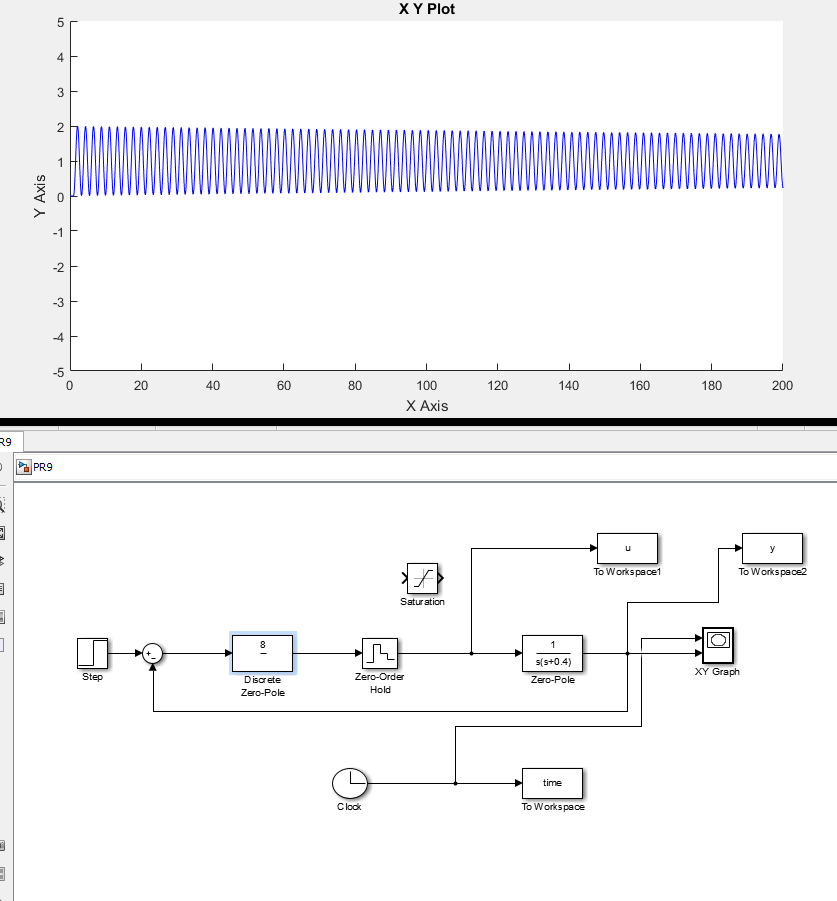
\includegraphics[width=0.8\textwidth]{stable.png}
    \caption{A barely stable gain for this system}
\end{figure}
\begin{figure}[H]
    \centering
    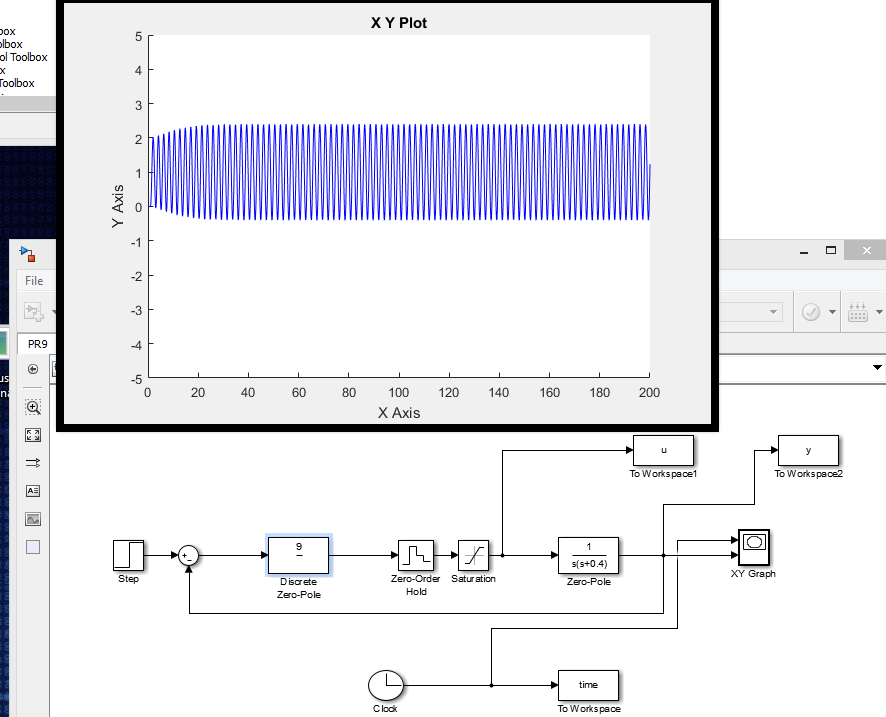
\includegraphics[width=0.8\textwidth]{unstable.png}
    \caption{An unstable gain for this system}
\end{figure}
Then I used a saturation block and saw that it forced the system to be marginally stable as seen below.
\begin{figure}[H]
    \centering
    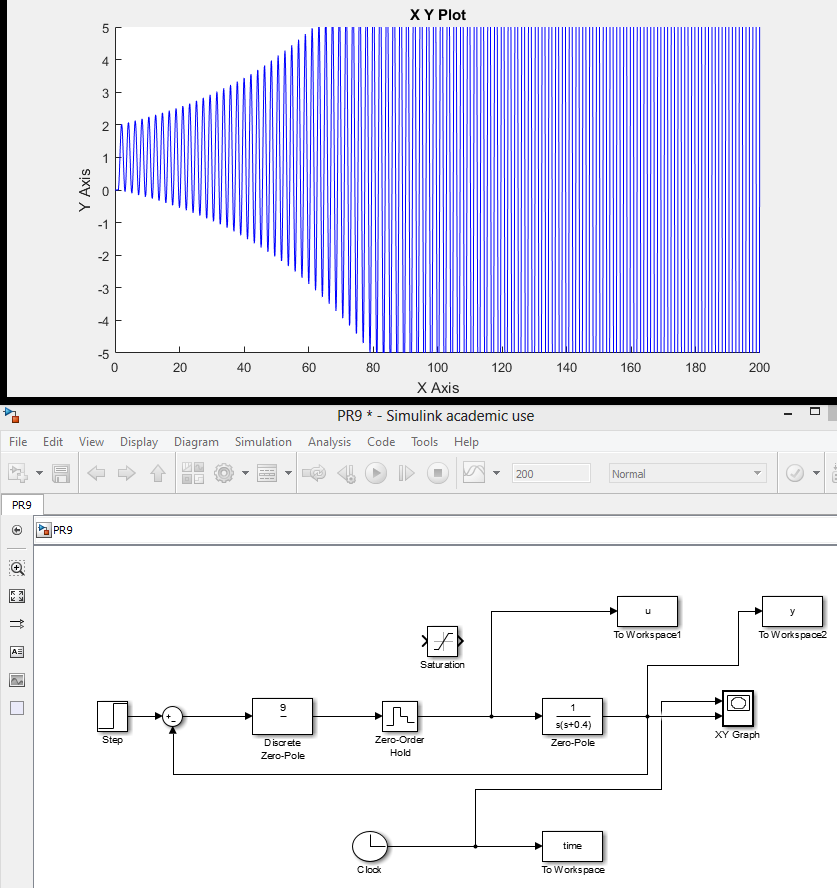
\includegraphics[width=0.8\textwidth]{unstable_nosat.png}
    \caption{An unstable gain with Saturation making it marginally stable once it hits saturation}
\end{figure}
To determine what exact value of $k_1$ results in an unstable gain, we must find the discrete closed loop transfer function for this system and determine what gain gives the poles a magnitude of 1. Anything above that gain will be unstable. The zero-order hold discrete transfer function is:
\[G(z)=\cfrac{0.004934z+0.004869}{z^2-1.961z+0.9608}\]
The closed loop is then:
\[GC(z)=\cfrac{k_1G(z)}{1+k_1G(z)}=\cfrac{k_1(0.004934*z+0.004869)}{z^2+(k_10.004934-1.961)z+0.9608+k_10.004869}\]
We need to know what gain forces one of the poles to be equal in magnitude to 1. Set the denominator equal to 1 and then solve for the k that gives that value. I tried doing this in Matlab with fsolve, but got the wrong answer consistently. The other option is to use the rootlocus and determine what gain results in a pole who's magnitude is 1. The plot of this is below.
\begin{figure}[H]
    \centering
    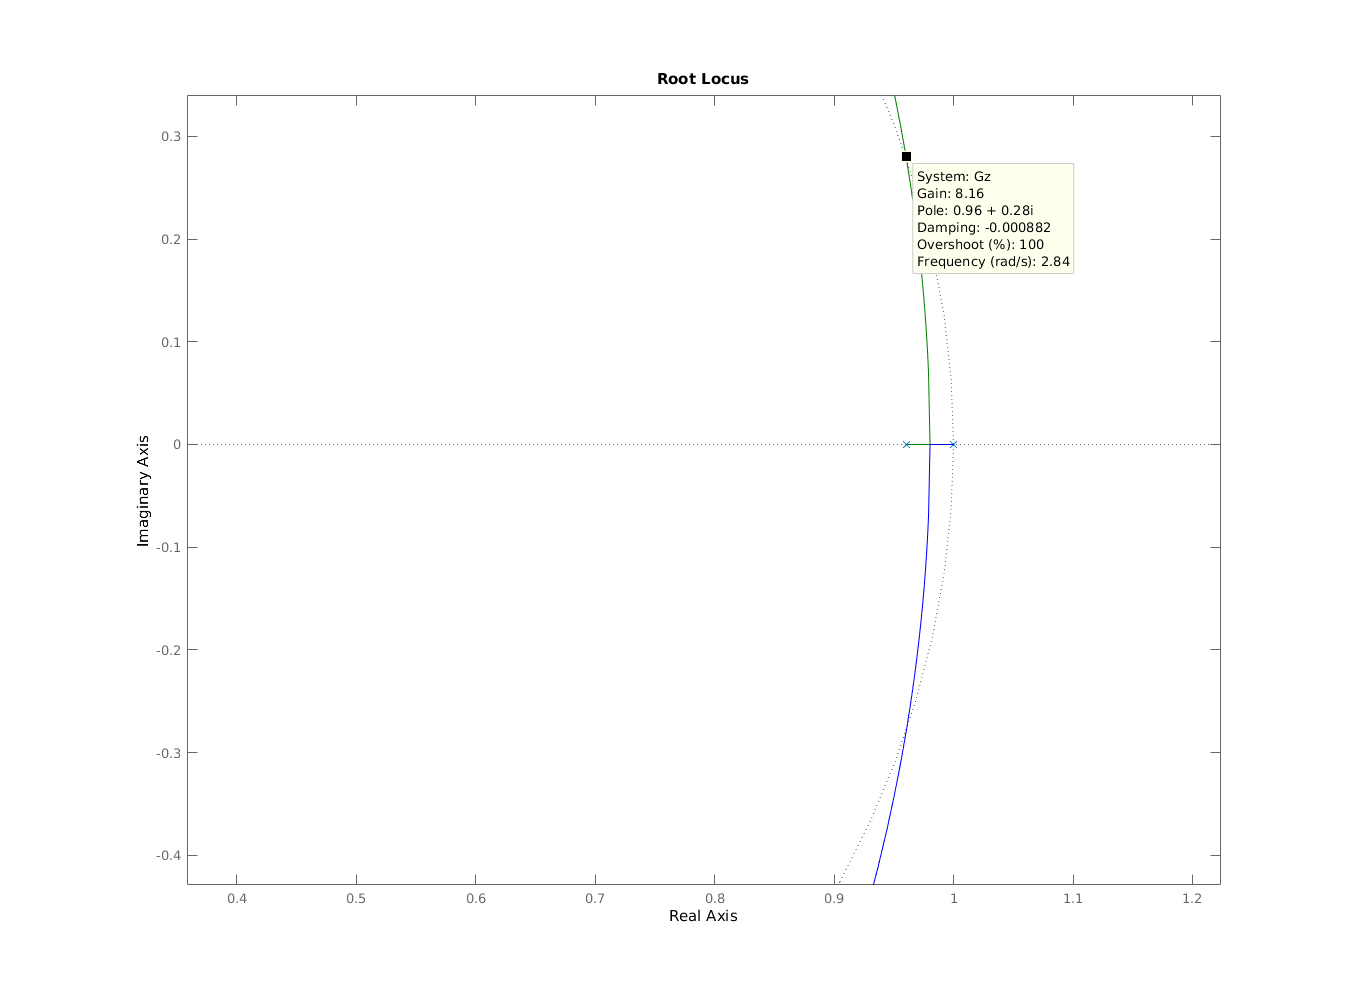
\includegraphics[width=0.8\textwidth]{rlocus.png}
\end{figure}

\end{document}
